\subsection{Sparsely distributed sensor arrays}
Sparsely distributed sensor arrays refer to layouts that limit the number of available sensors either by environmental parameters or by design. 
\subsubsection{3D location tracking}
 \begin{figure}[h]
\centering
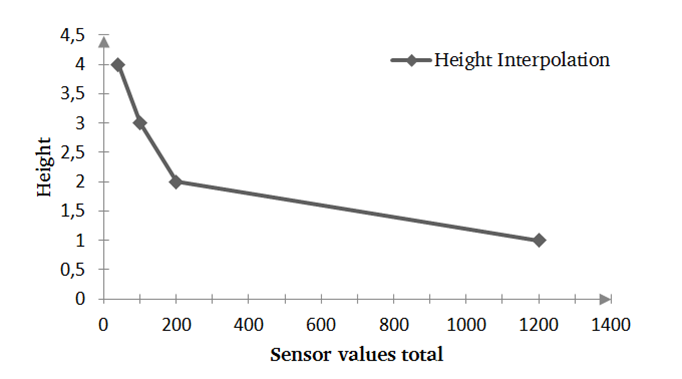
\includegraphics[width=0.6\textwidth]{images/magicbox_data_zaxis}
\caption{Piecewise linear hand distance estimation \cite{Braun2011MultiInputDevice}}
\label{fig:magicbox_data_zaxis}
\end{figure}
%Figure 29 Piecewise linear hand distance estimation [78]
The first data processing step of the MagicBox is the planar localization of the hand, following the weighted average algorithm previously presented. In order to calculate the distance of the hand from the plane we are using a piecewise linear interpolation, that resembles the response curve of a single sensor \cite{Braun2011MultiInputDevice}.
\begin{figure}[h]
\centering
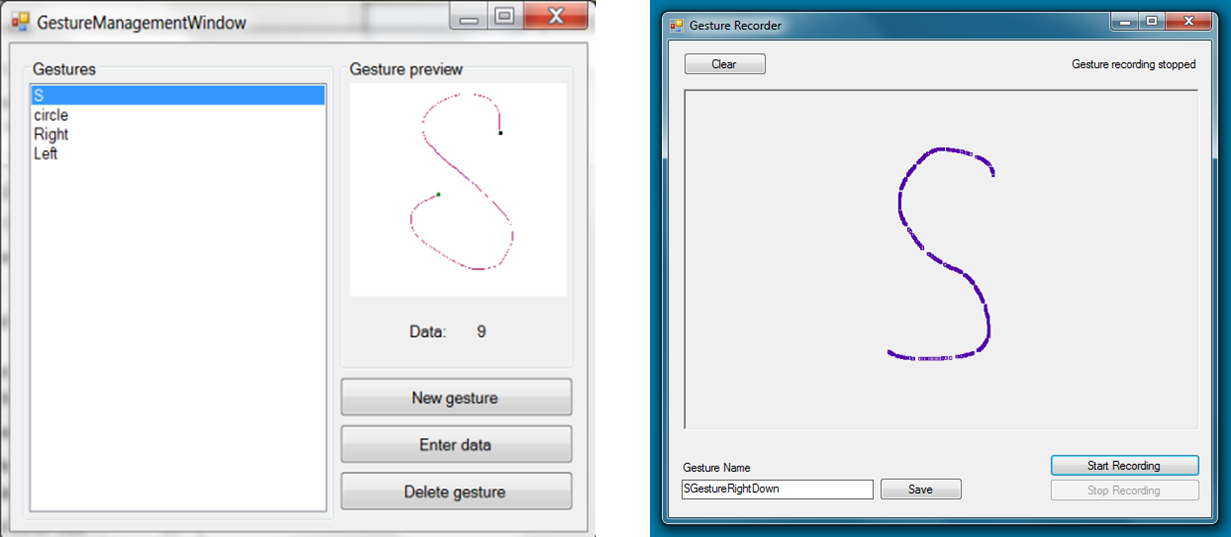
\includegraphics[width=0.7\textwidth]{images/magicbox_data_gest}
\caption{Gesture overview module (left) and gesture recorder (right)}
\label{fig:magicbox_data_gest}
\end{figure}
%Figure 30 Gesture overview module (left) and gesture recorder (right)
An addition of the MagicBox was a generic gesture recognition module based on methods similar to mouse gesture recognition \cite{braun2013capacitive}, albeit adapted for three dimensional locations. The developed debug software allows defining an arbitrary set of potential gestures and adding training data, as shown in Figure \ref{fig:magicbox_data_gest}. The module is looking for matches based on the most recent set of locations. 
The general functionality of a gesture recognition framework that is using learning by example is shown in Figure 1. A set of features is extracted from incoming raw data. These are distributed to training sets that are used to associate certain features to given gestures. After this learning process is completed current feature sets that are acquired on-the-fly are tested against the training features in the repository. If certain criteria are met, these lookups lead to successfully recognized gestures and
subsequently, an action may be performed. 

Figure 2 - Gesture recognition framework layer model
Our proposed framework is implementing gesture recognition by example, employing a multi-level design as shown in Figure 2. The lowest level - User Control - is a collection of aspects that are controllable by the user. The Algorithm Control allows setting the parameters of the gesture recognition algorithm, Current Feature allows selecting between different methods of feature acquisition from the raw data and Current Gestures is the set of gestures that
can be recognized. The Object Level is encompassing all objects in the frameworks, the group of gesture recognition algorithms the user can choose from and their current settings. Furthermore, there are the available features including settings and the set of available gestures. Above is the Module Management Level that controls feature acquisition and gesture management on a contextual level, meaning that, based on the current situation, the framework can select different features and gestures to process. Finally the Framework Management Level is controlling high-
level functionality of all modules and provides interfaces to external applications to control the framework and access registered gestures.
The framework is implemented in the Microsoft .NET environment (version 4.0) using C\#. It requires a gesture
recognition device that provides location data in three dimensions.
In our cases this is an array of capacitive proximity sensors that will be detailed in the prototype section.
Figure 3 - Screenshots of gesture manager and gesture
recorder
The key aspect of gestures by example – providing examples - is realized in a debug application. It provides a simple way to record exemplary movements and associate them to gesture sets. The main screens realizing this functionality are shown in Figure 3.
On the left side we can see the management screen that allows
adding and deleting of gestures, as well as a preview window that is an average of the sample data associated to this gesture. The process of entering data is shown on the right side where several samples can be recorded and associated to the selected gesture and the user can decide, whether the current movement should be stored or discarded.
\subsubsection{Large-area location tracking}
Using long wire electrodes may result in considerable noise and influence from outside electric fields. Therefore CapFloor requires preprocessing to reduce the noise and achieve a more robust high-level data processing. The localization uses the weighted average algorithm that has been presented previously. 
\begin{figure}[h]
\centering
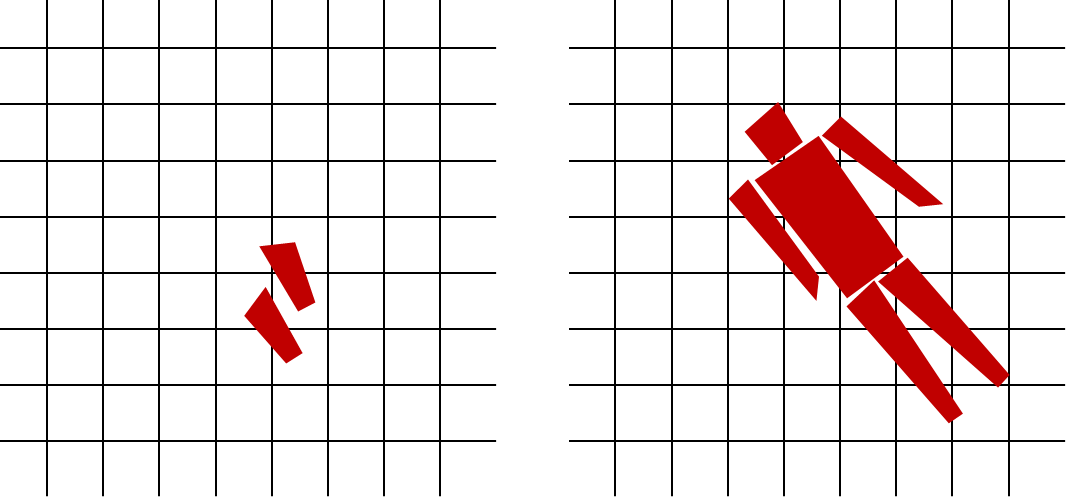
\includegraphics[width=0.8\textwidth]{images/floor_shapes}
\caption{Shapes of a standing and lynig person on top of the CapFloor grid}
\label{fig:capfloor_shapes}
\end{figure}
The fall detection is using a time-series analysis of the aggregated values of the sensors that are currently detecting an object. This method is using the assumption that the overall sensor response is roughly equivalent to the shape of the object that is closest to the surface, resulting in a higher capacitance of the overall system, similar to the plate capacitor model. This effect is shown in Figure \ref{fig:capfloor_shapes}. The sum $s$ of all n sensor values $r$ is the closest equivalent to the system capacitance and therefore a viable measure. If the overall value is beyond a certain threshold $v_l$ we can consider a lying person $p_l$.
\begin{equation}
s=\sum^n_{i=0}{r_i}\ \ \ ,\ \ \ p_l=\left\{ \begin{array}{c}
1,\ \ \ s\ge v_l \\ 
0,\ \ \ s<v_l \end{array}
\right.
\end{equation}
In order to increase the robustness this threshold has to be exceeded for a certain amount of time $t_m$. In consequence a fall $f$ is detected if the following equation is 1.
\begin{equation}
f=\prod^{t_m}_{j=0}{p_{l,t_j}}
\end{equation}